\begin{pastexam}[label={px:df3-103-ds-02}]{地方三等資訊處理 103 年 第二題}
（申論；20 分）

給定一個二元樹 T。若 T 之後序巡行（postorder traversal）結果是 P D J M O A I H K G L N E B C，而中序巡行
（inorder traversal）結果是 J D P I A M O C K H G B E L N：
\begin{itemize}[leftmargin=2.2em, nosep]
\item[㈠] 請畫出該二元樹 T。（10 分）
\item[㈡] 請寫出該二元樹之前序巡行（preorder traversal）結果。（10 分）
\end{itemize}
\end{pastexam}

\begin{pastsoln}
答案：㈠ 樹畫在下面。 ㈡ 前序是 C I J D P A O M B G K H E N L。

\textbf{㈠ 重建}（資結書第~7.4~節、定理~7.4）：後序的最後一個是根；在中序裡找到根，左邊是左子樹、右邊是
右子樹；後序裡前面同樣個數的是左子樹、接著是右子樹。 遞迴拆下去：
\begin{itemize}
\item 根 $C$。 中序 $C$ 左邊 J D P I A M O（$7$ 個）是左子樹，右邊 K H G B E L N 是右子樹；後序前 $7$ 個
P D J M O A I 是左子樹，接著 H K G L N E B 是右子樹。
\item 左子樹：後序最後是 $I$，根 $I$。 中序 J D P $\mid$ I $\mid$ A M O。
\begin{itemize}
\item $I$ 的左子樹：後序 P D J、中序 J D P。 根 $J$，中序 $J$ 在最前面，沒有左子樹；右子樹後序 P D、中序
D P，根 $D$，$P$ 是 $D$ 的右子節點。
\item $I$ 的右子樹：後序 M O A、中序 A M O。 根 $A$，沒有左子樹；右子樹後序 M O、中序 M O，根 $O$，$M$ 是
$O$ 的左子節點。
\end{itemize}
\item 右子樹：後序 H K G L N E B，根 $B$。 中序 K H G $\mid$ B $\mid$ E L N。
\begin{itemize}
\item $B$ 的左子樹：後序 H K G、中序 K H G。 根 $G$，中序 $G$ 在最後，沒有右子樹；左子樹後序 H K、中序 K H，
根 $K$，$H$ 是 $K$ 的右子節點。
\item $B$ 的右子樹：後序 L N E、中序 E L N。 根 $E$，沒有左子樹；右子樹後序 L N、中序 L N，根 $N$，$L$ 是
$N$ 的左子節點。
\end{itemize}
\end{itemize}
\begin{center}
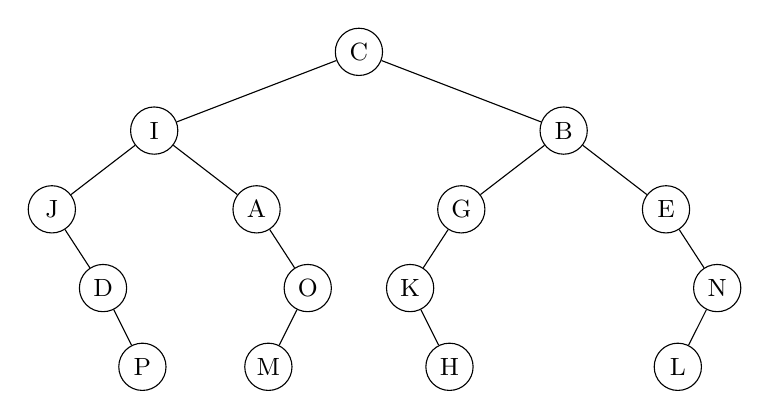
\begin{tikzpicture}[every node/.style={circle,draw,minimum size=6mm,inner sep=0pt,font=\small},
  level distance=10mm, level 1/.style={sibling distance=52mm}, level 2/.style={sibling distance=26mm},
  level 3/.style={sibling distance=13mm}, level 4/.style={sibling distance=10mm}]
\node {C}
  child {node {I}
    child {node {J} child[missing] child {node {D} child[missing] child {node {P}}}}
    child {node {A} child[missing] child {node {O} child {node {M}} child[missing]}}}
  child {node {B}
    child {node {G} child {node {K} child[missing] child {node {H}}} child[missing]}
    child {node {E} child[missing] child {node {N} child {node {L}} child[missing]}}};
\end{tikzpicture}
\end{center}
中序加後序可以唯一決定一棵二元樹（資結書定理~7.4 的對稱版本），所以這棵樹是唯一的。 檢查：這棵樹的中序是
J D P I A M O C K H G B E L N，後序是 P D J M O A I H K G L N E B C，都和題目相同。

\textbf{㈡ 前序}（根、左、右）：$C$，左子樹 $I\ J\ D\ P\ A\ O\ M$，右子樹 $B\ G\ K\ H\ E\ N\ L$：
\[
\text{C I J D P A O M B G K H E N L}.
\]
\end{pastsoln}
